%%%%%%%%%%%%%%%%%%%
% MOTIVATION
%%%%%%%%%%%%%%%%%%%
\def\title{Motivation: Question Answering}
\begin{frame}{\title}
\begin{center}
  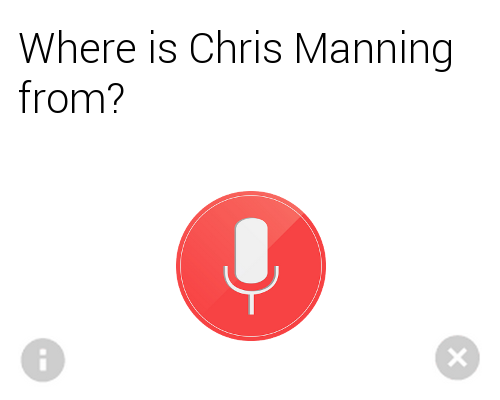
\includegraphics[width=7cm]{../../img/google-chris-manning-origin.png}
\end{center}
\end{frame}

\begin{frame}[noframenumbering]{\title}
\vspace{-1cm}
\begin{center}
  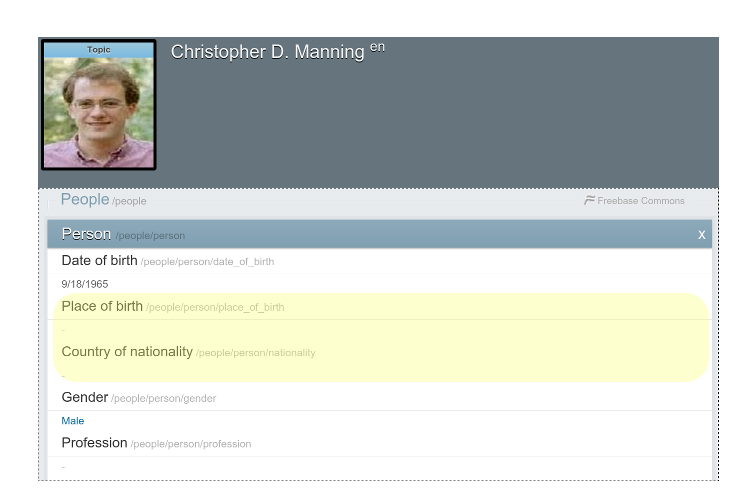
\includegraphics[width=10.5cm]{../../img/chris-freebase.png}
\end{center}
\end{frame}

\begin{frame}[noframenumbering]{\title}
\begin{center}
  \begin{tabular}{l}
  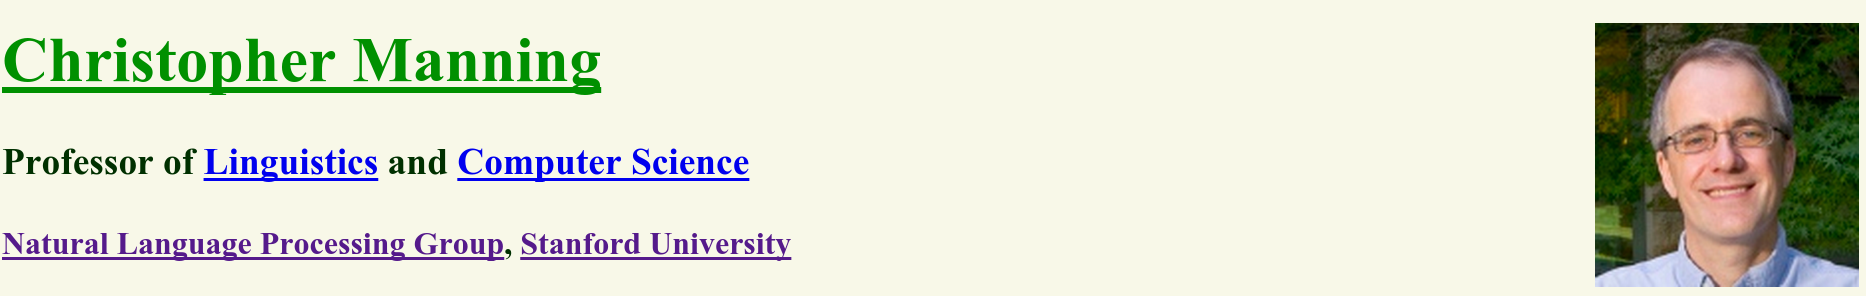
\includegraphics[width=12cm]{../../img/chris-website-header.png} \\
  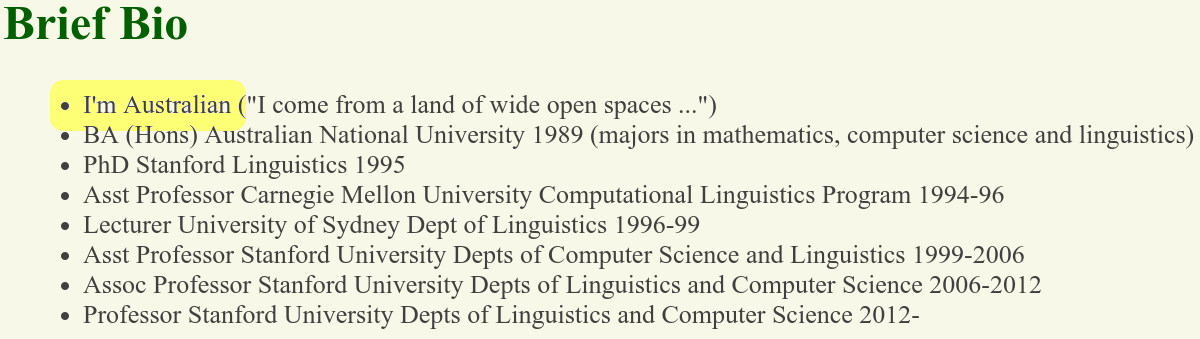
\includegraphics[width=9cm]{../../img/chris-bio.png}
  \end{tabular}
\end{center}
\end{frame}
\begin{frame}[noframenumbering]{\title}
\begin{center}
  \fbox{
\includegraphics[width=7cm]{../../img/google-chris-manning-origin-answer.png}}
\end{center}
\end{frame}

%%%%%%%%%%%%%%%%%%%
% K-WAY CLASSIFICATION
%%%%%%%%%%%%%%%%%%%
\def\title{Relation Extraction}
\begin{frame}{\title}
\hh{Input}:  Sentences containing (\subj{subject}, \obj{object}). \\
\hh{Output}: \rel{Relation} between \subj{subject} and \obj{object}. \\
\vspace{1em}
\pause

\begin{center}
  \w{\subj{I} 'm \obj{Australian}} $\implies$ \rel{per:origin}
\end{center}
\pause

\begin{center}
  \includegraphics[height=4cm]<1-2>{../../img/hammer-placeholder.jpg}
  \includegraphics[height=4cm]<3-3>{../../img/hammer.jpg}
  \includegraphics[height=4cm]<4-4>{../../img/hammer-name.jpg}
\end{center}
\end{frame}

%%%%%%%%%%%%%%%%%%%
% OPEN DOMAIN REL MOTIVATION
%%%%%%%%%%%%%%%%%%%
\def\title{What about...}
\begin{frame}{\title}
\begin{center}
  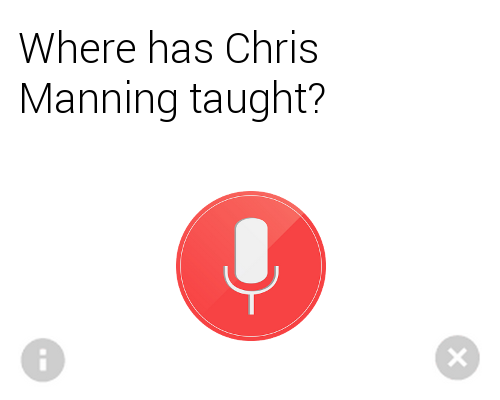
\includegraphics[width=7cm]{../../img/google-chris-manning-taught.png}
\end{center}
\end{frame}
\begin{frame}[noframenumbering]{\title}
\begin{center}
  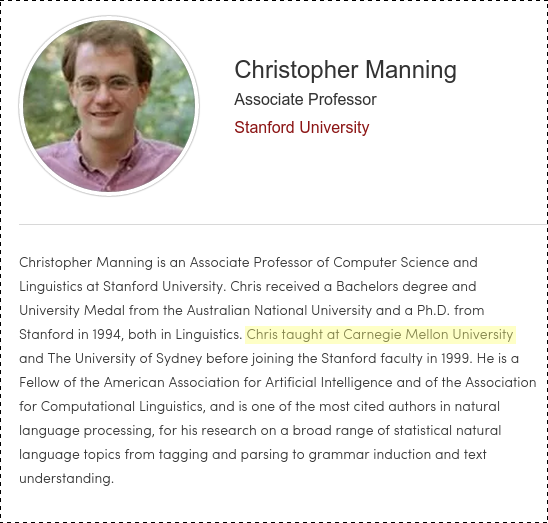
\includegraphics[height=7cm]{../../img/chris-coursera-taught.png} \\
\end{center}
\end{frame}
\begin{frame}[noframenumbering]{\title}
\begin{center}
  
\includegraphics[width=7cm]{../../img/google-chris-manning-research.png}
\end{center}
\end{frame}
\begin{frame}[noframenumbering]{\title}
\begin{center}
  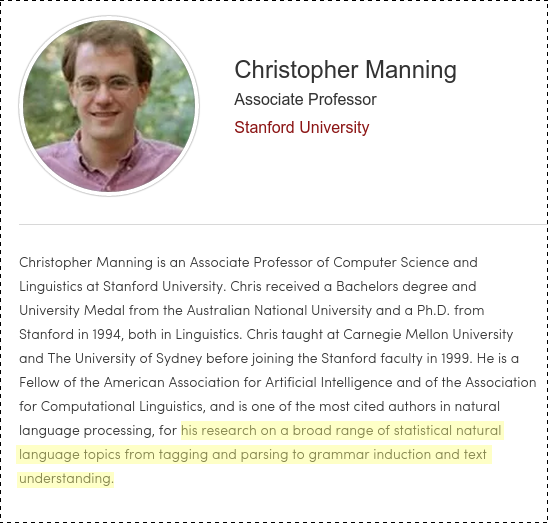
\includegraphics[height=7cm]{../../img/chris-coursera-research.png} \\
\end{center}
\end{frame}

%%%%%%%%%%%%%%%%%%%
% OPEN IE
%%%%%%%%%%%%%%%%%%%
\def\title{Open Information Extraction}
\begin{frame}{\title}
\begin{center}
  \hh{Extract \textit{arbitrary} relations over \textit{arbitrary} entities} \\
\end{center}
\vspace{1em}
\pause

(\subj{Chris}, \rel{taught at}, \obj{Carnegie Mellon}) \\
(\subj{Chris}, \rel{taught at}, \obj{University of Sydney}) \\
(\subj{his research}, \rel{is on}, \obj{A broad range of statistical natural language topics})
\pause

(\subj{Obama}, \rel{was born in}, \obj{Hawaii}) \\
(\subj{young rabbits}, \rel{drink}, \obj{milk}) \\
(\subj{Heinz Fischer}, \rel{visits}, \obj{United States}) \\
\vspace{1em}
\pause

\hh{Open IE is not new}
\begin{itemize}
  \item UW: TextRunner, ReVerb, Ollie, OpenIE 4, ImplIE
  \item CMU: NELL
\end{itemize}
\end{frame}


%%%%%%%%%%%%%%%%%%%
% CHALLENGE: LONG SENTENCES
%%%%%%%%%%%%%%%%%%%
\def\title{Challenge: Long Sentences}
\begin{frame}{\title}
\hh{Short sentences are easy:}
\begin{center}
  \begin{dependency}[text only label,label style={above}]
    \begin{deptext}[column sep=-0.00cm]
      Obama \& was \& born \& in \& Hawaii \&[-1ex] . \\
    \end{deptext}
    \depedge[edge unit distance=2.25ex]{3}{5}{nmod:in}
    \depedge[edge unit distance=1.5ex]{3}{2}{cop}
    \depedge[edge unit distance=2.25ex]{3}{1}{nsubj}
    \depedge[edge unit distance=1.5ex]{5}{4}{case}
  \end{dependency}
\end{center}
\pause

\hh{But most sentences are longer:}
\begin{center}
  \begin{dependency}[text only label, label style={above}]
    \begin{deptext}[column sep=-0.00cm]
      Born \& in \& a \& small \& town \&[-1ex] , \& she \& took \& the \&
        midnight \& train \& going \& anywhere \&[-1ex] . \\
    \end{deptext}
    \depedge[edge unit distance=1.75ex]{1}{5}{nmod:in}
    \depedge[edge unit distance=1.5ex]{5}{4}{amod}
    \depedge[edge unit distance=2.25ex]{5}{3}{det}
    \depedge[edge unit distance=1.4ex]{8}{1}{vmod}
    \depedge[edge unit distance=2.5ex]{8}{7}{nsubj}
    \depedge[edge unit distance=2.25ex]{8}{11}{dobj}
    \depedge[edge unit distance=1.5ex]{11}{10}{nn}
    \depedge[edge unit distance=1.9ex]{11}{9}{det}
    \depedge[edge unit distance=1.5ex]{11}{12}{vmod}
    \depedge[edge unit distance=1.5ex]{12}{13}{dobj}
  \end{dependency}
\end{center}
\end{frame}


%%%%%%%%%%%%%%%%%%%
% CHALLENGE: LOST CONTEXT
%%%%%%%%%%%%%%%%%%%
\def\title{Challenge: Lost Context}
\def\deletable#1{\darkred{\hbox{\transparent{0.75} #1}}}
\begin{frame}{\title}
\hh{Sometimes annoying:}
\begin{center}
  \begin{dependency}[text only label,label style={above}]
    \begin{deptext}[column sep=-0.00cm]
      She \& was \& born \& in \& the \& small \& town \& 
      \deletable{of} \& \deletable{Springfield} \&[-1ex] . \\
    \end{deptext}
    \depedge[edge unit distance=2.25ex]{3}{1}{nmod:in}
    \depedge[edge unit distance=2.0ex]{3}{2}{cop}
    \depedge[edge unit distance=2.0ex]{3}{7}{nmod:in}
    \depedge[edge unit distance=2.25ex]{7}{6}{amod}
    \depedge[edge unit distance=2.5ex]{7}{5}{det}
    \depedge[edge unit distance=2.25ex,edge style={darkred!100!black,thick}]{7}{9}{nmod:of}
  \end{dependency}
\end{center}
\pause

\hh{Sometimes logically invalid:}
\begin{center}
  \begin{dependency}[text only label, label style={above}]
    \begin{deptext}[column sep=-0.00cm]
      All \& \deletable{young} \& rabbits \& drink \& milk \&[-1ex] . \\
    \end{deptext}
    \depedge[edge unit distance=1.75ex]{4}{3}{nsubj}
    \depedge[edge unit distance=1.75ex]{4}{5}{dobj}
    \depedge[edge unit distance=1.75ex,edge style={darkred!100!black,thick}]{3}{2}{amod}
    \depedge[edge unit distance=2.5ex]{3}{1}{det}
  \end{dependency}
\end{center}
\end{frame}

%%%%%%%%%%%%%%%%%%%
% CHALLENGE: TOO MUCH CONTEXT
%%%%%%%%%%%%%%%%%%%
\def\title{Challenge: Too Much Context}
\begin{frame}{\title}
\begin{center}
  \begin{dependency}[text only label, label style={above}]
    \begin{deptext}[column sep=-0.00cm]
      Heinz \& Fischer \& of \& Austria \& visits \& the \& United \& States \&[-1ex] . \\
    \end{deptext}
    \depedge[edge unit distance=2.00ex]{5}{2}{nsubj}
    \depedge[edge unit distance=2.25ex]{5}{8}{dobj}
    \depedge[edge unit distance=1.75ex]{2}{1}{nn}
    \depedge[edge unit distance=1.50ex]{2}{4}{nmod:of}
    \depedge[edge unit distance=1.75ex]{8}{7}{nn}
    \depedge[edge unit distance=2.00ex]{8}{6}{det}
  \end{dependency}

  (\subj{Heinz Fischer of Austria}; \rel{visits}; \obj{the United States})
\end{center}

\hh{Is this about Heinz Fischer or Austria?}
\pause
\begin{itemize}
  \item Is the subject a PERSON or ORGANIZATION? \\
        (\subj{United States president Obama}; \rel{visits}; \obj{China})
  \pause
  \item Downstream applications don't want to deal with this.
  \item Downstream applications have less context to figure this out.
\end{itemize}
\end{frame}
